%%%%%%%%%%%%%%%%%%%%%%%%%%%%%%%%%%%%%%%%%%%%%%%%%%%%%%%%%%%%%%%%%%%%%
% LaTeX Template: Project Titlepage Modified (v 0.1) by rcx
%
% Original Source: http://www.howtotex.com
% Date: February 2014
% 
% This is a title page template which be used for articles & reports.
% 
% This is the modified version of the original Latex template from
% aforementioned website.
% 
%%%%%%%%%%%%%%%%%%%%%%%%%%%%%%%%%%%%%%%%%%%%%%%%%%%%%%%%%%%%%%%%%%%%%%

\documentclass[12pt]{report}
\usepackage[a4paper]{geometry}
\usepackage[myheadings]{fullpage}
\usepackage{fancyhdr}
\usepackage{lastpage}
\usepackage{graphicx, wrapfig, subcaption, setspace, booktabs}
\usepackage[english]{babel}
\usepackage{color}
\usepackage{hyperref}
\usepackage{array}
\usepackage{supertabular}
\usepackage{hhline}
\usepackage{enumitem}
\usepackage[T1]{fontenc}
\usepackage[utf8]{inputenc}
\usepackage{graphicx}

\newcommand{\HRule}[1]{\rule{\linewidth}{#1}}
\renewcommand{\theenumii}{\arabic{enumii}.}
\addto\captionsenglish{
  \renewcommand{\contentsname}
    {Innhold}
}
\onehalfspacing
\setcounter{tocdepth}{5}
\setcounter{secnumdepth}{5}

%-------------------------------------------------------------------------------
% HEADER & FOOTER
%-------------------------------------------------------------------------------
\pagestyle{fancy}
\fancyhf{}
\setlength\headheight{15pt}
\fancyhead[L]{Team D} 
\fancyhead[R]{Universitetet i Bergen}
\fancyfoot[R]{Page \thepage\ of \pageref{LastPage}}
%-------------------------------------------------------------------------------
% TITLE PAGE
%-------------------------------------------------------------------------------

\begin{document}

\title{ \normalsize \textsc{}
		\\ [2.0cm]
		\HRule{0.5pt} \\
		\LARGE \textbf{\uppercase{Matkrig}}
		\HRule{2pt} \\ [0.5cm]
		\normalsize \today \vspace*{5\baselineskip}}

\date{}

\author{
		Team D  \\ 
		Universitetet i Bergen \\
		Informatikk }

\maketitle
\tableofcontents
\newpage

%-------------------------------------------------------------------------------
% BODY
%-------------------------------------------------------------------------------

\section*{Bruksm{\o}nstertekst:}
\addcontentsline{toc}{section}{Bruksm{\o}nstertekst:}

\textbf{Tittel}: Eliminere motstandere
\bigskip \\
\textbf{Akt{\o}rer}: Spillere, system
\bigskip \\
\textbf{Prim{\ae}rakt{\o}r}: Spiller
\bigskip \\
\textbf{Tid}: 30 sek per spiller, runden varer i 10-15 min
\bigskip \\
\textbf{M{\aa}l}: Kvitte seg med med alle motstandere
\bigskip \\
\textbf{Pre-conditions:} Spillet er startet p{\aa} en datamaskin

\subsubsection*{Hovedflyt:}
\begin{enumerate}
\item Akt{\o}r n f{\aa}r 30 sekunder p{\aa} {\aa} bevege seg fritt p{\aa} kartet. 
\item Akt{\o}r n velger v{\aa}pen 
\item Akt{\o}r n velger retning 
\item Akt{\o}r n velger kraft for lenge
\item Systemet registrer prosjektilposisjon 
\item Systemet endrer milj{\o}et ut ifra prosjektilkraft og type 
\item Motstander blir truffet av prosjektil 
\item Systemet beregner motstanders helse minus skaden som ble utgjort
\item Motstander mister helsepoeng 
\item Motstander d{\o}r
\item Gjenst{\aa}ende spiller vinner
\end{enumerate}

\subsubsection*{Alternativ handlinger:}

\begin{enumerate}[label=\Alph*]
\item 
\bigskip

\begin{enumerate}
\item @1 Akt{\o}r beveger seg ut av kartet 
\item Gjenoppta @11 
\end{enumerate}
\item 
\bigskip

\begin{enumerate}
\item @2 Akt{\o}r har ikke ammunisjon 
\item Gjenoppta @2 
\end{enumerate}
\item 
\bigskip

\begin{enumerate}
\item @9 Motstander overlever 
\item Gjenoppta @1 
\end{enumerate}
\item 
\bigskip

\begin{enumerate}
\item @Everywhere Rundetiden g{\aa}r ut 
\item Akt{\o}r med mest gjenst{\aa}ende helsepoeng vinner
\end{enumerate}
\item 
\bigskip

\begin{enumerate}
\item @2 Tid for {\aa} velge v{\aa}pen/retning/kraft g{\aa}r ut 
\item Akt{\o}r f{\aa}r ikke angrepet 
\item Gjenoppta @1
\end{enumerate}
\end{enumerate}

\section*{Bruksm{\o}nsterdiagram:}
\addcontentsline{toc}{section}{Bruksm{\o}nsterdiagram:}

\vspace{4cm}
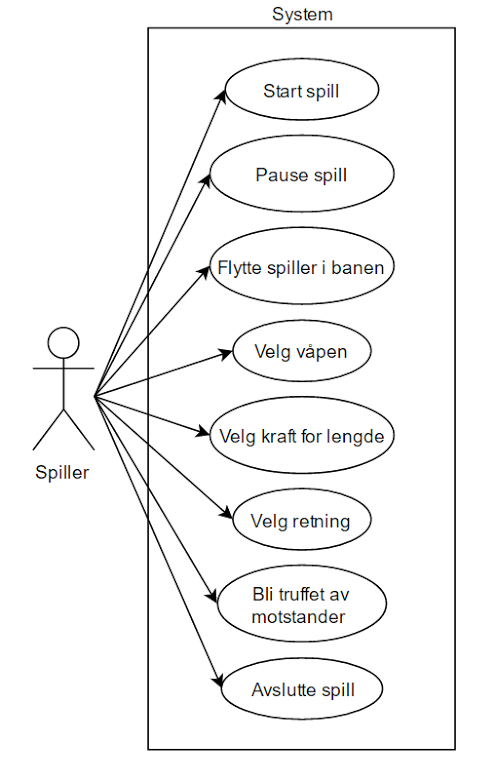
\includegraphics[width=0.8\textwidth,natwidth=500,natheight=642]{use_case_diagram_m.png}

\end{document}